\subsubsection{Change outfit}
Sơ đồ use-case Change outfit:
\begin{figure}[H]
    \centering
    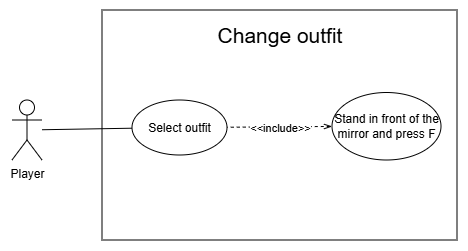
\includegraphics[width=0.75\linewidth]{4.Đặc tả chi tiết các lược đồ/Use-case/images/ChangeOutfit.png}
    \caption{Use-case mô tả Change outfit}
    \label{fig:placeholder}
\end{figure}


\begin{table}[H]
\centering
\begin{tabular}{|p{4cm}|p{10cm}|}
\hline
\textbf{Use-case name} & Change outfit \\ \hline
\textbf{Actor} & Người chơi \\ \hline
\textbf{Descriptions} & Use-case này sẽ chỉ ra các bước cần thực hiện để có thể thay đổi trang phục. \\ \hline
\textbf{Pre-conditions} & Phải vào được trong lobby \\ \hline
\textbf{Trigger} & Không có. \\ \hline
\textbf{Post-conditions} & Không có \\ \hline
\textbf{Normal Flow} &
\begin{enumerate}
\item Người chơi di chuyển đến trước gương.
\item Người chơi nhấn giữ \textbf{''F''} để vào trang thái thay trang phục.
\item Người chơi chọn trang phục mình muốn bằng cách nhấn các mũi tên tương ứng với loại trang phục.
\item Người chơi nhấn giữ \textbf{''F''} để thoát trạng thái thay trang phục.
\item Use-case kết thúc sau khi người chơi thoát trạng thái thay trang phục.
\end{enumerate}
\\ \hline
\textbf{Alternative Flow} &
Không có
\\ \hline
\textbf{Exception Flow} &
Không có
\\ \hline
\end{tabular}
\end{table}